%!TEX program=xelatex
\documentclass{article}

% Chinese font
\usepackage{xeCJK}
\usepackage{hyperref}

\setCJKmainfont{[kaiu.ttf]}
\setmainfont{[times new roman.ttf]}

\usepackage{colortbl}
\usepackage{xcolor}

\definecolor{LightGray}{gray}{0.8}
\newcolumntype{a}{>{\columncolor{LightGray}}c}

\usepackage{tabularx}
\usepackage{makecell}
\usepackage{graphicx}
\graphicspath{{./img/}}

\usepackage{indentfirst}

\renewcommand*\contentsname{目錄}

\begin{document}
\begin{titlepage}
	\centering

	{\huge 海大教室借用平台}

	\vfill

	{\huge 設計文件}

	\vfill

	\begin{Large}
		\begin{center}
			\begin{tabular}{| a | c |}
				\hline
				專案名稱 & 海大教室借用平台               \\ \hline
				撰寫日期 & \today                 \\ \hline
				發展者  & \makecell{曾昱翔、林暐傑、陳鈺翔、 \\張銀軒、黃見弘} \\ \hline
			\end{tabular}
		\end{center}
	\end{Large}
\end{titlepage}


\addcontentsline{toc}{section}{版次變更紀錄}
\section*{版次變更紀錄}

\begin{tabularx}{\textwidth}{| c | X | X |}
	\rowcolor{LightGray}
	\hline
	版次  & 變更項目 & 變更日期       \\ \hline
	0.1 & 初版   & 2022/10/04 \\ \hline
	0.2 & 增加User Interface Design 部分& 2022/11/20   \\ \hline
	    &      &            \\ \hline
	    &      &            \\ \hline
	    &      &            \\ \hline
	    &      &            \\ \hline
\end{tabularx}

\newpage

\begin{center}
	\tableofcontents
\end{center}

\newpage

\section[系統模型與架構(SYSTEM MODEL/SYSTEM ARCHITECTURE)]{系統模型與架構(System Model/System Architecture)}

\newpage

\section[介面需求與設計(INTERFACE REQUIREMENTS AND DESIGN)]{介面需求與設計(Interface Requirements and Design)}

\newpage

\section[流程設計(PROCESS DESIGN)]{流程設計(Process Design)}

\newpage

\section[使用者畫面設計(USER INTERFACE DESIGN)]{使用者畫面設計(User Interface Design)}

	\bigskip
	\begin{Large}
		註冊頁面
	\end{Large}
	
	\begin{center}
		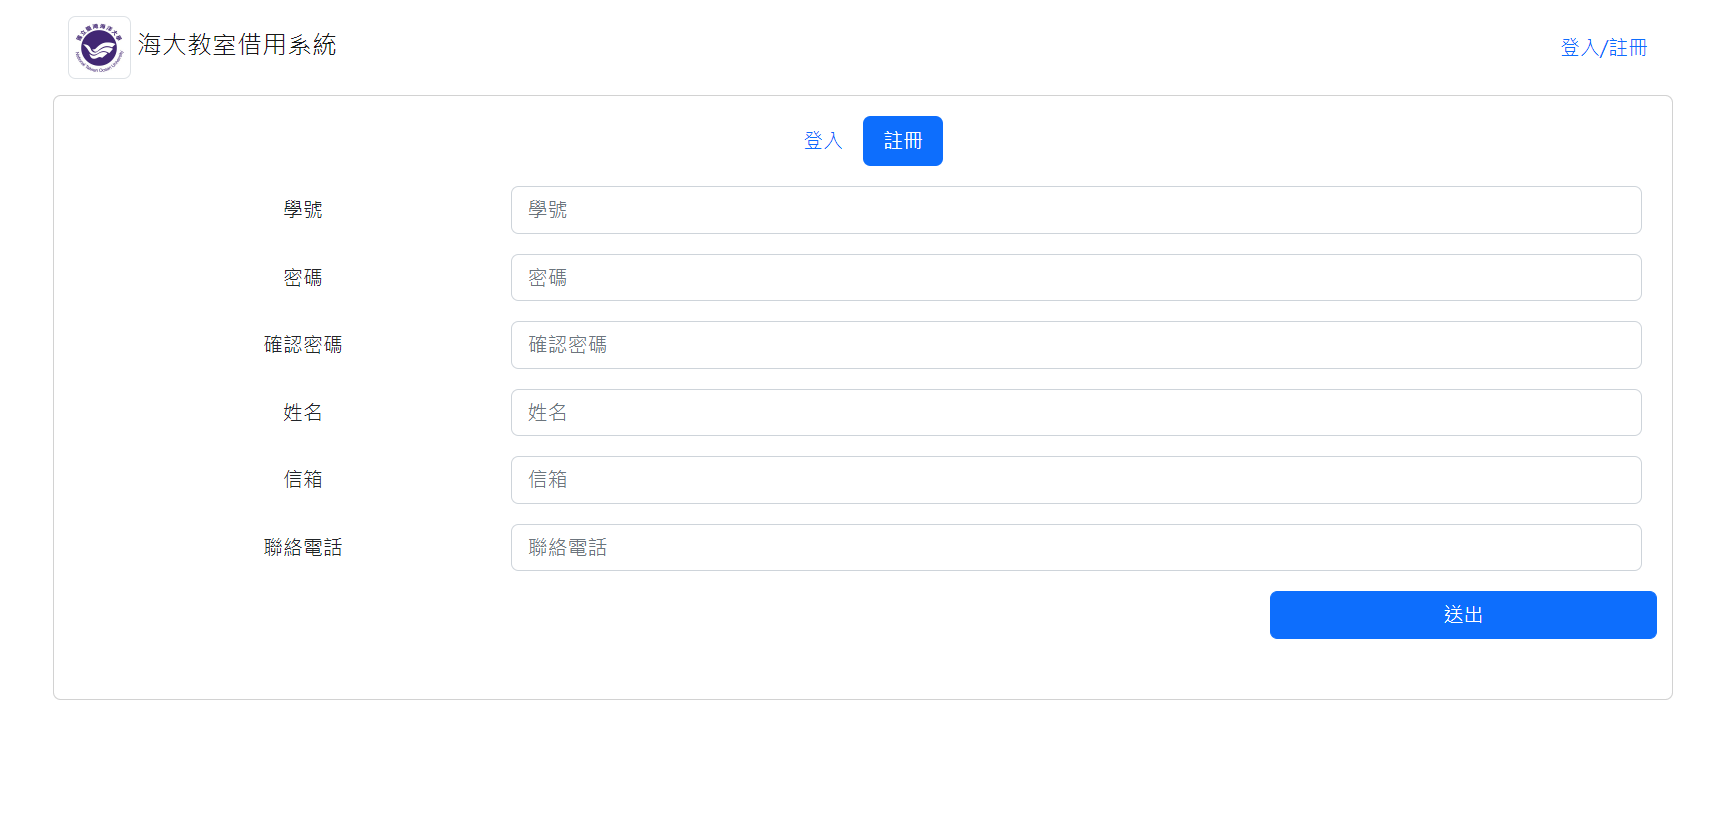
\includegraphics[height=0.35\textheight]{SDDRegister.png}
	\end{center}
	使用者註冊時須提供學號、姓名、信箱、聯絡電話等資訊註冊,待管理員核可後即可登入本系統。

	\bigskip
	\bigskip
	\begin{Large}
		登入頁面
	\end{Large}

	\begin{center}
		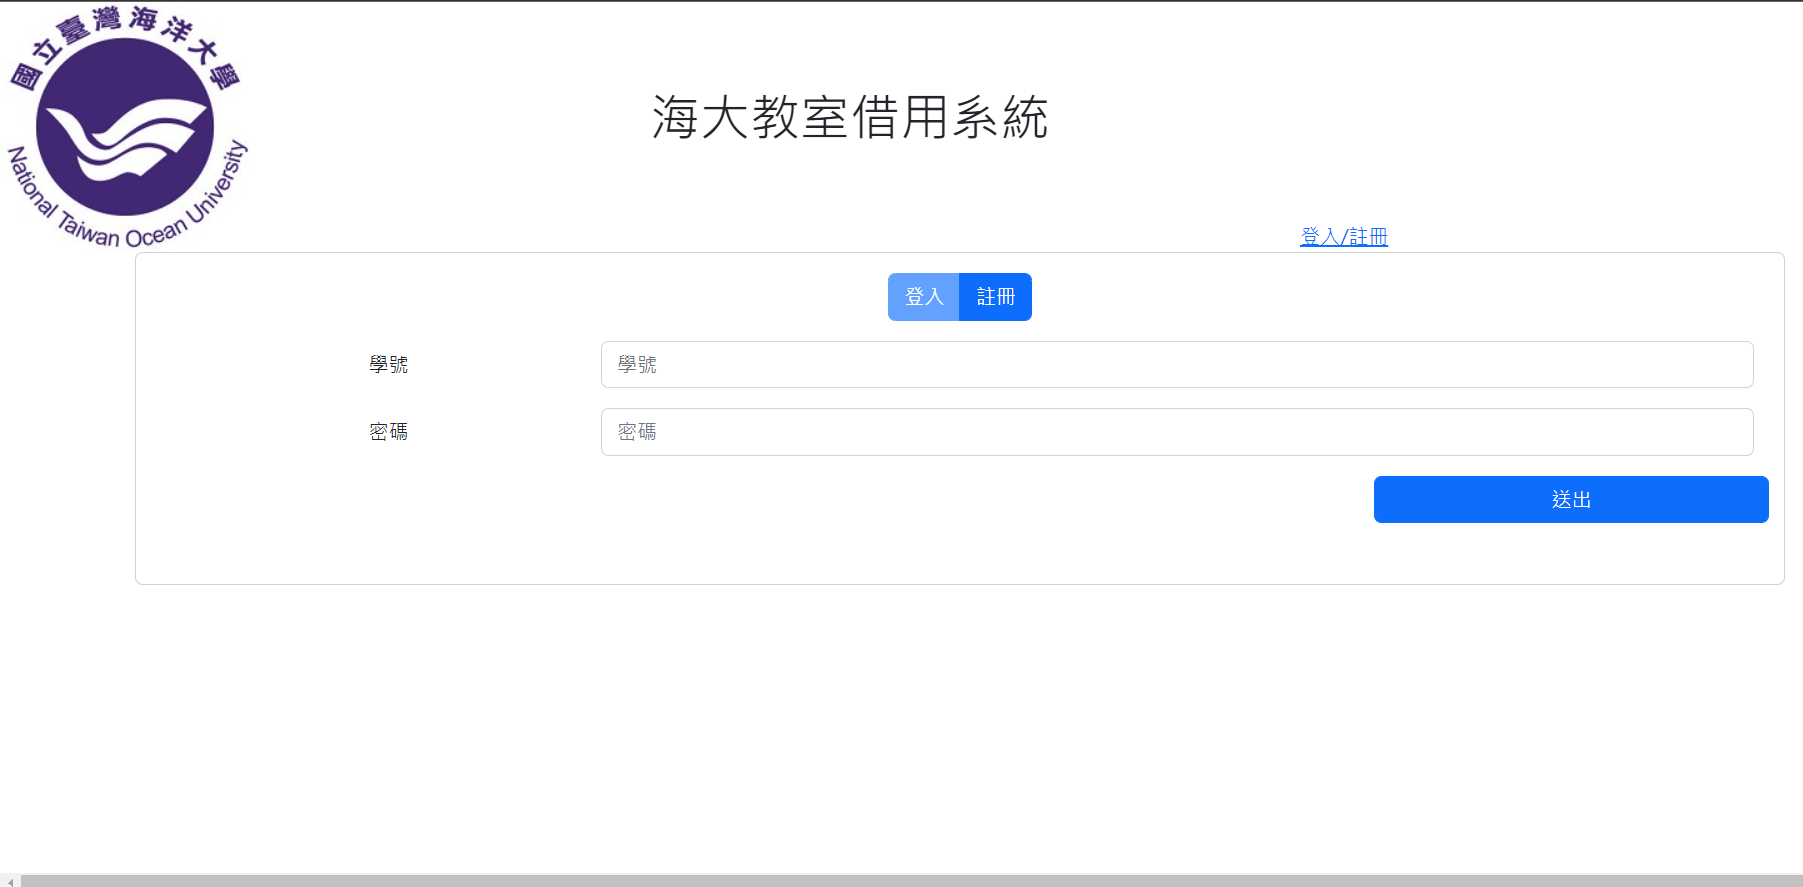
\includegraphics[height=0.35\textheight]{SDDLogin.png}
	\end{center}
	在使用者註冊後,需輸入註冊時所使用的學號及密碼登入。
\newpage


\begin{Large}
	未登入首頁
\end{Large}
\bigskip
\begin{center}
	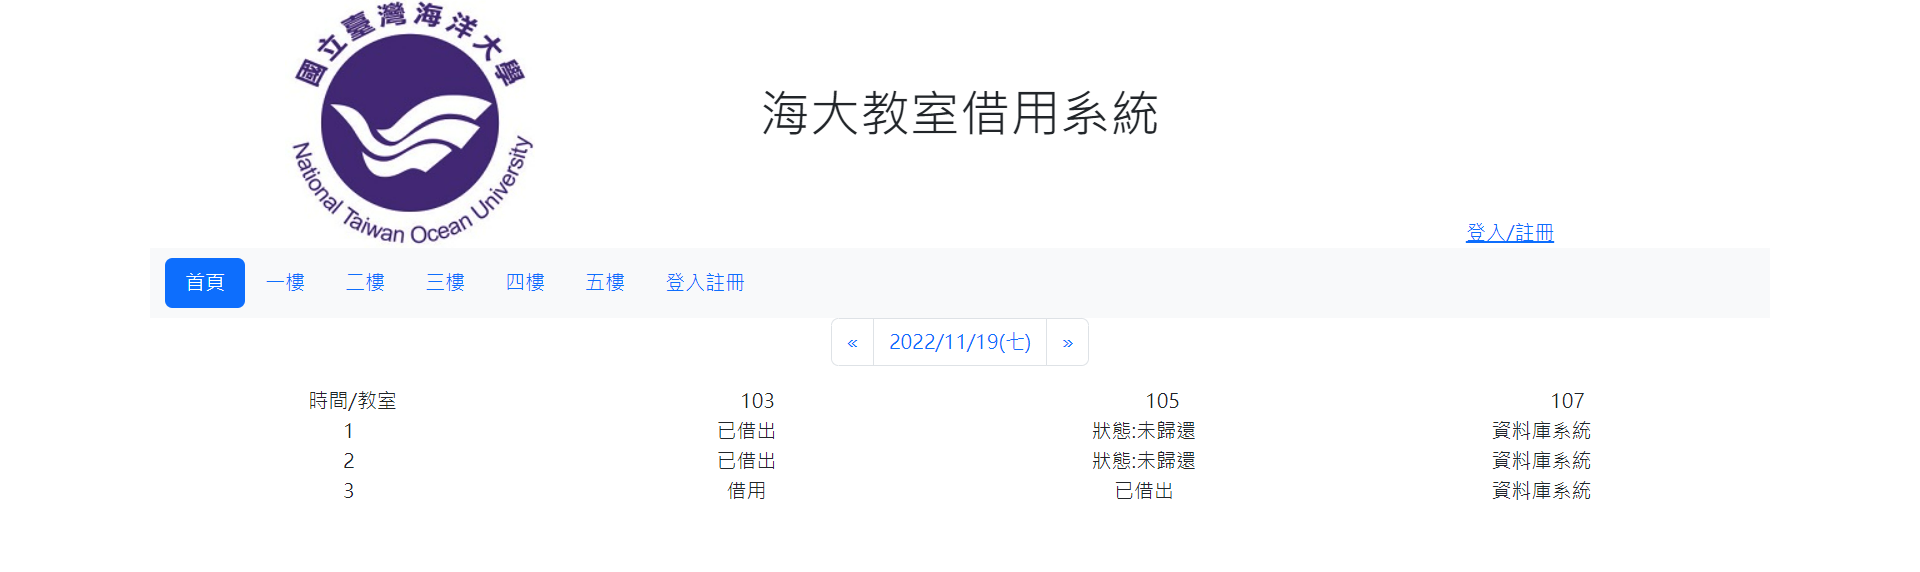
\includegraphics[scale=0.35]{SDDFirstpage.png}
\end{center}
	左上角logo : 按下後跳回首頁。
	\bigskip
 \\ 導覽列     : 此處可選擇欲借教室(選擇樓層->選擇教室),也可登入/註冊帳號。
 	\bigskip
 \\ 中間區塊   : 日期可調整,選定後即會跳出教室該日的借用及歸還狀況。
 
\bigskip
\bigskip
\bigskip
\bigskip
\bigskip
\hspace*{\fill} 

\begin{Large}
	使用者登入首頁
\end{Large}
\bigskip
\begin{center}
	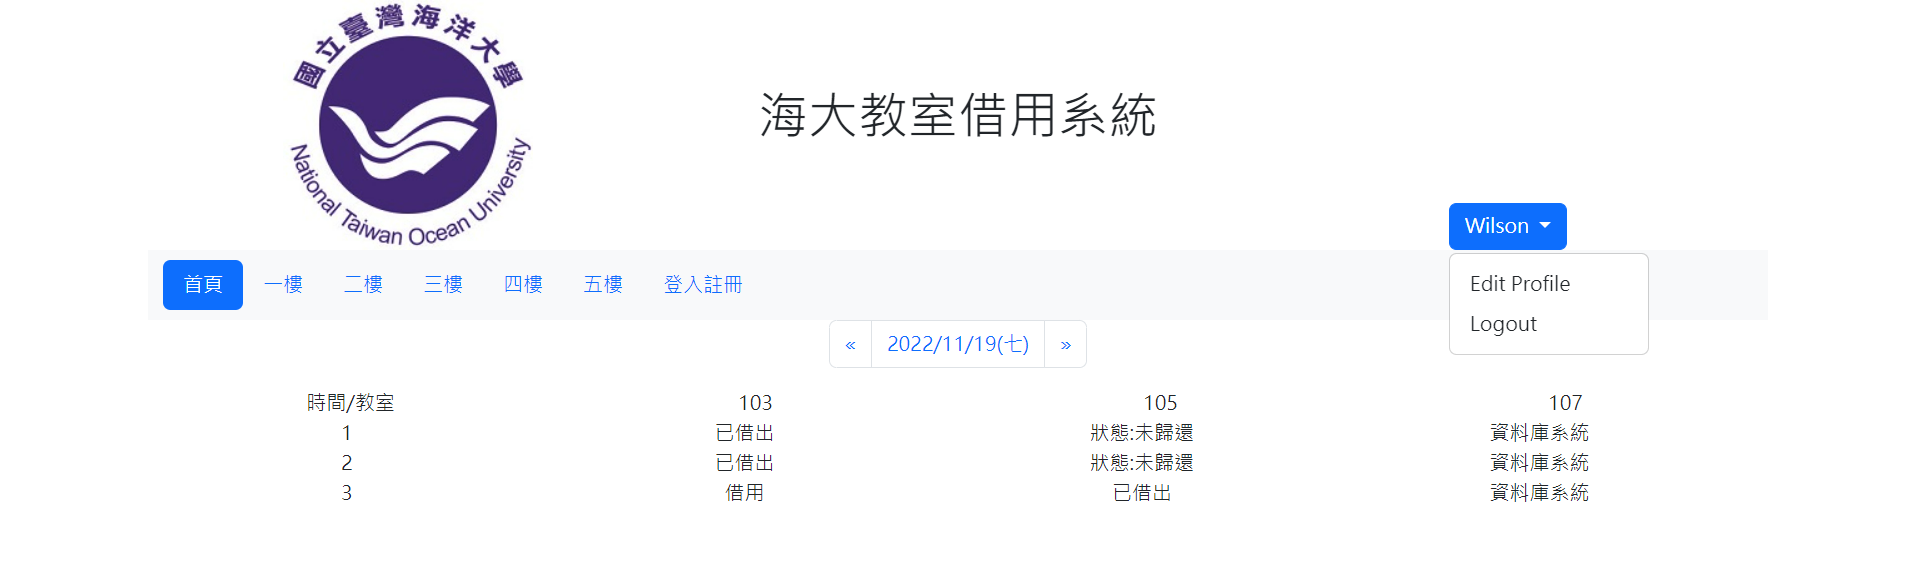
\includegraphics[scale=0.35]{SDDUserLoginnedFirstpage.png}
\end{center}
在註冊/登入後,右方會顯示使用者名稱,點擊後可選擇查看個人檔案或登出。
\bigskip
\newpage

\begin{Large}
	管理者登入首頁
\end{Large}
\bigskip
\begin{center}
	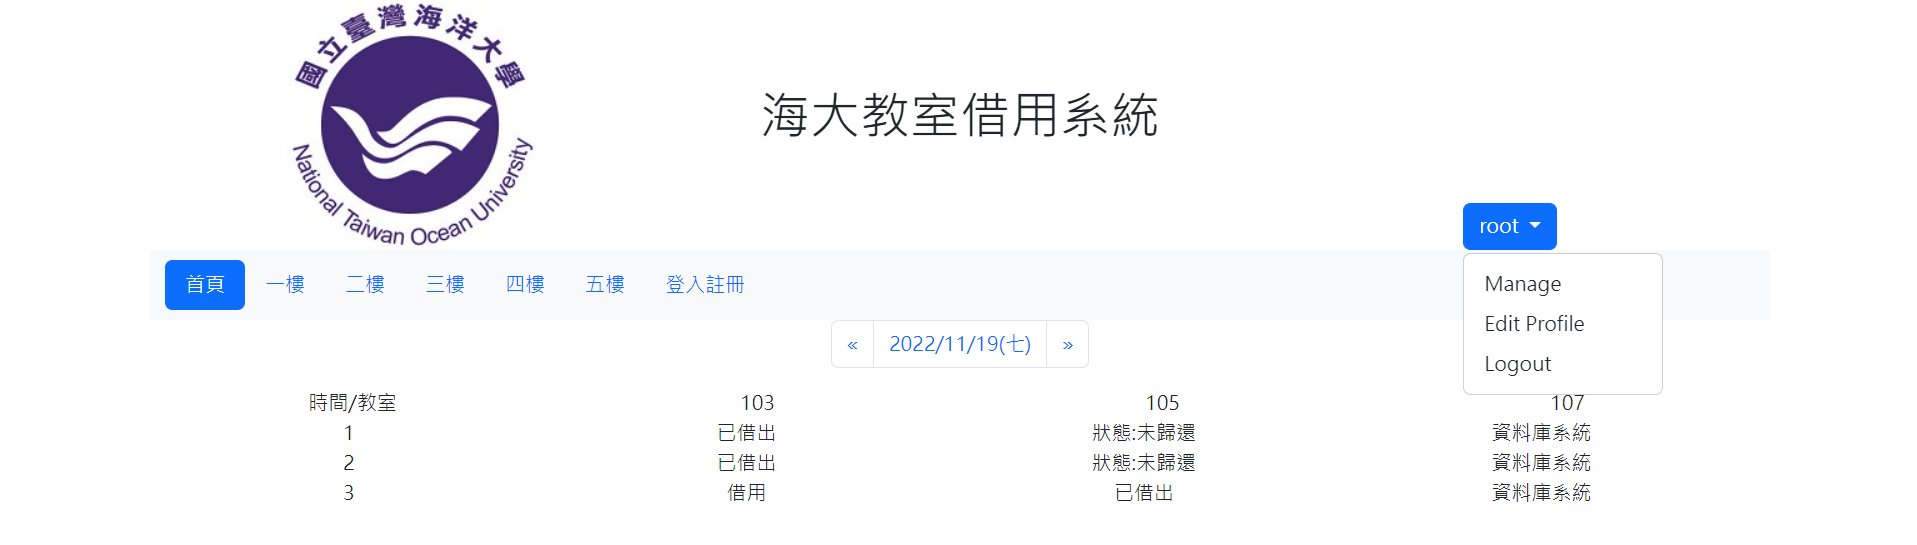
\includegraphics[scale=0.35]{SDDAdminLoginnedFirstpage.png}
\end{center}
\bigskip
\bigskip
當登入帳號為管理者帳號(root)時,右方會顯示root,點擊後可選擇進入管理者頁面、查看管理者檔案或登出。
\bigskip
\bigskip
\bigskip
\bigskip
\bigskip
\bigskip

\begin{Large}
	管理者頁面
\end{Large}
\bigskip
\begin{center}
	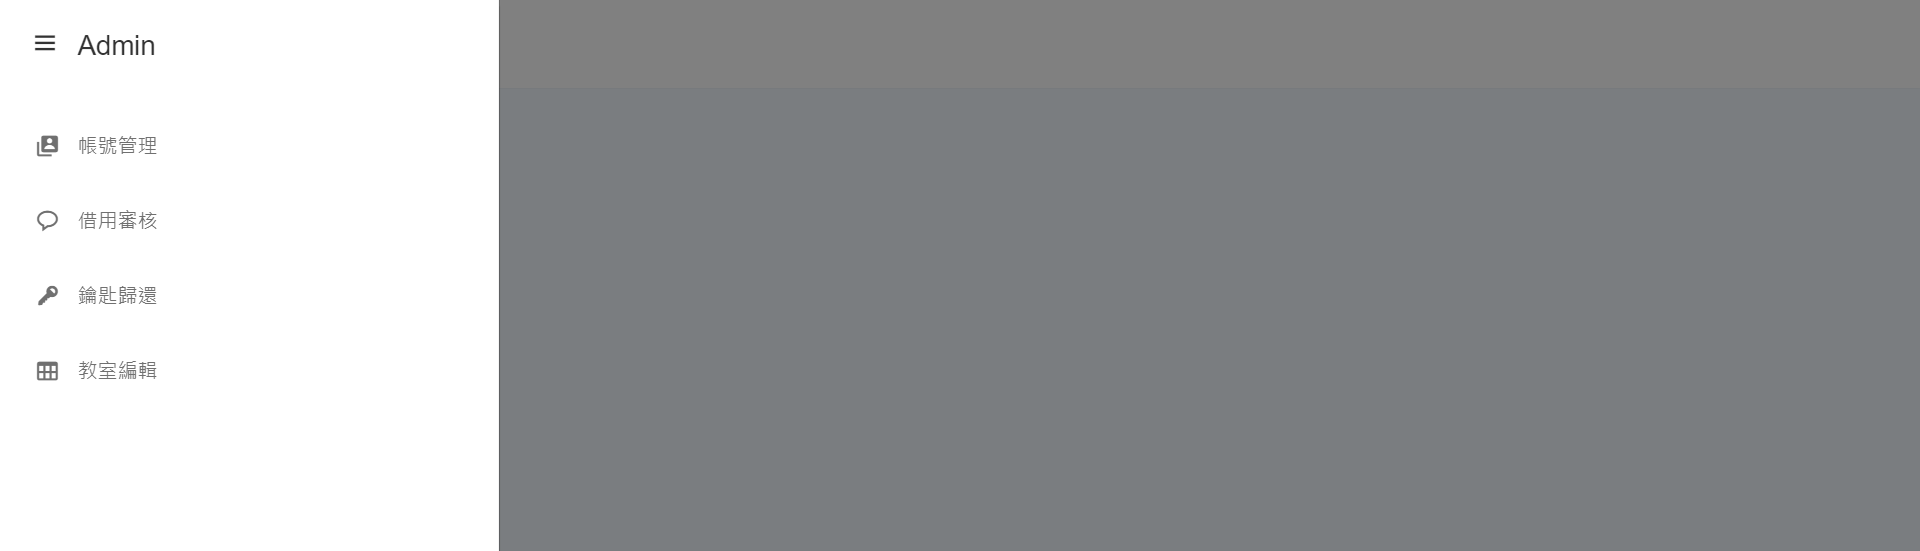
\includegraphics[scale=0.35]{SDDAdminPage.png}
\end{center}
\bigskip
\bigskip
在上個頁面中點選Manage後會進入管理者頁面,點開左上角後左側會滑出功能列,可選擇欲執行的功能。
\bigskip
\bigskip
\hspace*{\fill} 

\newpage

\begin{Large}
	帳號管理頁面
\end{Large}
\bigskip
\begin{center}
	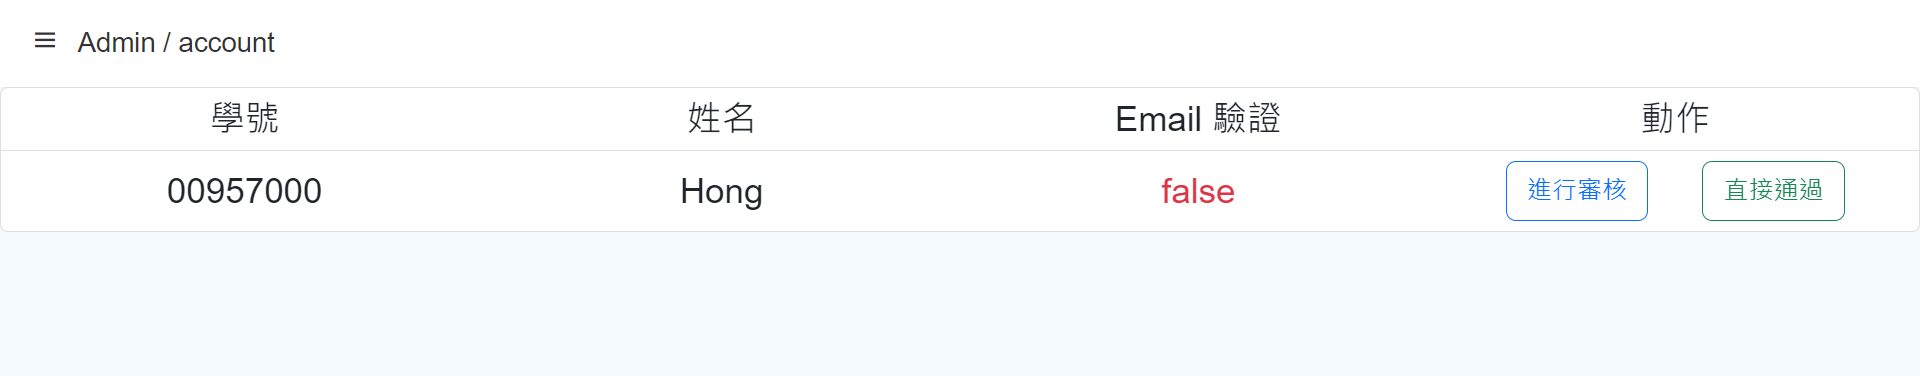
\includegraphics[scale=0.35]{SDDAdminAccountManage.png}
\end{center}
\bigskip
\bigskip
管理者可透過此頁面查看申請帳號,查看各申請帳號Email驗證是否通過,並選擇進行審核或直接通過。
\bigskip
\bigskip
\bigskip
\bigskip
\bigskip
\bigskip
\hspace*{\fill} 

\begin{Large}
	帳號審核頁面
\end{Large}
\bigskip
\begin{center}
	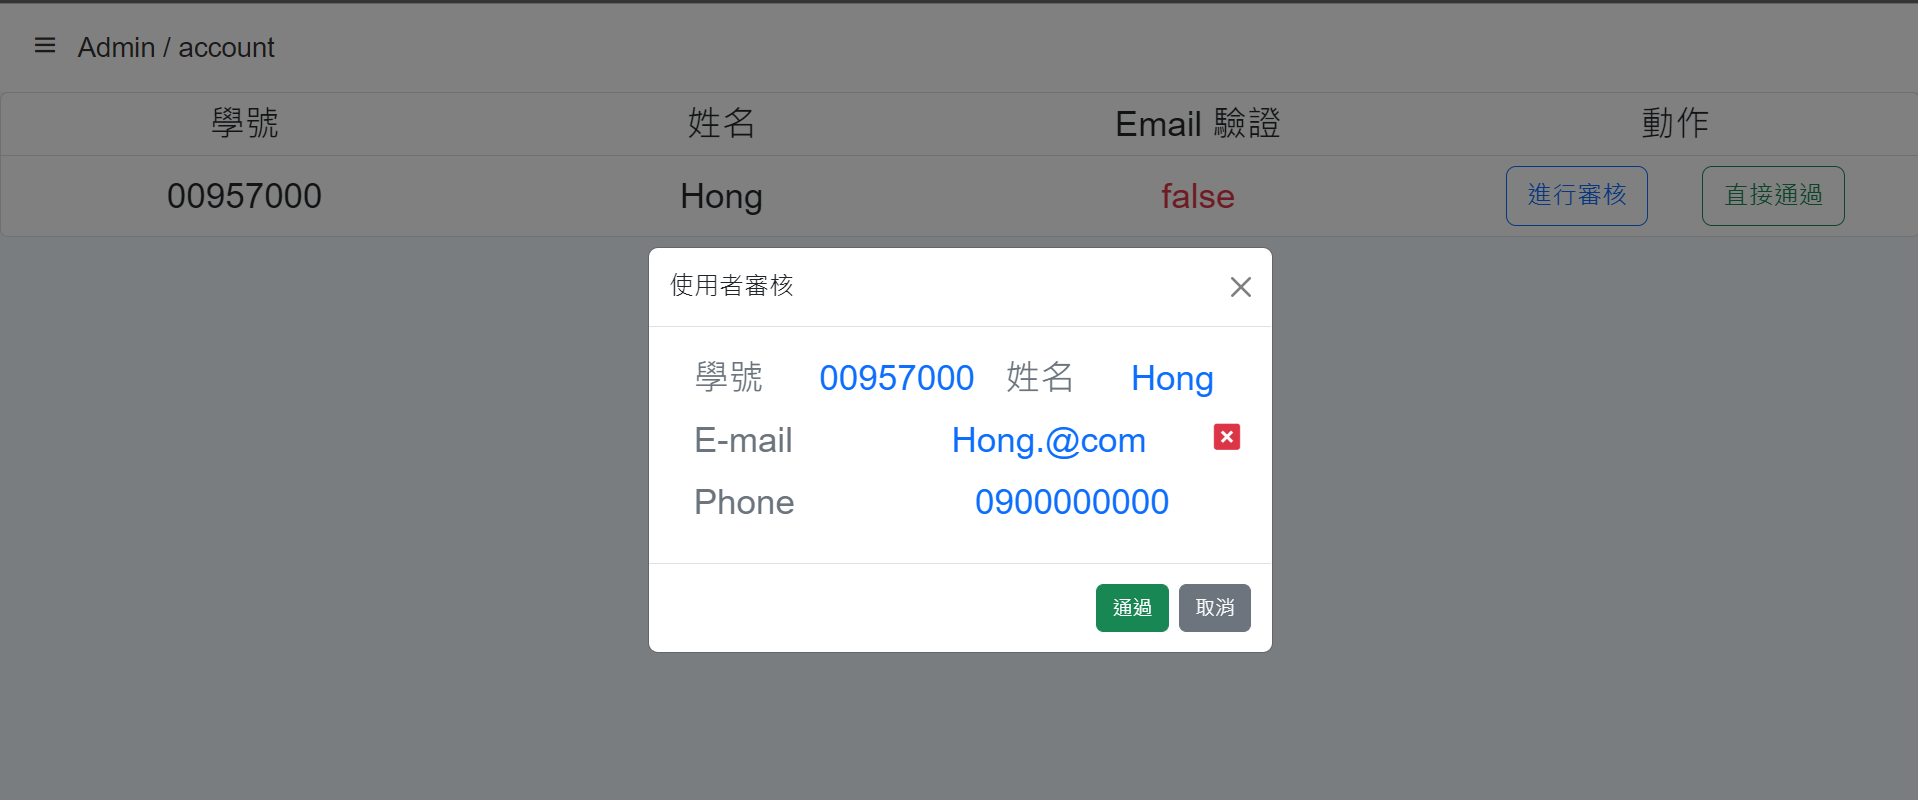
\includegraphics[scale=0.35]{SDDAdminAccountVerify.png}
\end{center}
\bigskip
\bigskip
管理者在此可看到申請人資料,並決定是否通過該申請。
\newpage

\section[資料設計(DATA DESIGN)]{資料設計(Data Design)}

\newpage

\section[類別圖設計(CLASS DIAGRAM DESIGN)]{類別圖設計(Class Diagram Design)}

\newpage

\section[實作技術(IMPLEMENTATION LANGUAGE AND PLATFORM)]{實作技術(Implementation Language and Platform)}

\newpage

\section[設計議題(DESIGN ISSUE)]{設計議題(Design Issue)}

\end{document}